% !TEX root= ../main.tex
\externaldocument{general_trimming}
\externaldocument{odd_paths}
\externaldocument{odd_vels}
\section{Inductive definitions}
\label{sec:Inductive definitions}
All the graph structures presented in this chapter so far can easily be defined inductively.
For instance, given some graph $\mathbf{G}=(G,N)$, let $V_1 \subseteq G \times G$ denote the set of all pairs of vertices related by our original vel-definition (Definition~\ref{def:vel}) where `trimmed' meant strictly non-branching.

We can define $V_1$ inductively in the following way, with $a$ and $b$ being arbitrary vertices from $G$.
\begin{align}
  \textbf{(BC):}&\quad N(a,b) \vee N(b,a) &\Rightarrow  V_1(a,b)\\
  \textbf{(IS):}&\quad \exists c \in N(a): (N(c) =\{d\} \wedge V_1(d,b)) &\Rightarrow V_1(a,b)
\end{align}
The symmetry in the base case is what makes this a definition of a vel and not a path, while the trimmed-ness gets expressed by the restrictions we set on vertex $c$ in the inductive step.
\subsection{The $V_2$ construction}
\label{sub:The V2 construction}
It is now  much easier to formally express the new, weaker concept of trimming.
Let $V_2 \subseteq G \times G$ be the set of all pairs of vertices related by our new vel-definition.
$V_2$ can be defined inductively in the following way, again with $a$ and $b$ as arbitrary vertices from $G$.
\begin{align}
  \textbf{(BC):}&\quad N(a,b) \vee N(b,a) &\Rightarrow V_2(a,b)\label{eq:V2_BC}\\
  \textbf{(IS):}&\quad \exists c \in N(a):
  \left ( \begin{tabular}{l}
  $\exists d \in N(c): V_2(d,b) \quad \wedge$\\
  $\forall d \in N(c): V_2(d,b) \vee V_2(d,a) \vee V_2(d,d)$
  \end{tabular} \right )
  &\Rightarrow V_2(a,b)\label{eq:V2_IS}
\end{align}
Comparing the two inductive definitions, it is easy to see that $V_2$ is a generalization of $V_1$.

The fact that $V_2(a,b) \;\Rightarrow\; \vdash \ol{ab}$ can now be proven inductively, showing that $V_2$ satisfies implication (1):
\begin{proof}
  Given a graph $G$ with two vertices $a$ and $b$ such that $V_2(a,b)$:

  Base case:
  If $N(a,b)$ or $N(b,a)$, then the NAND-clause $\ol{ab}$ will be an axiom and thus trivially provable.

  Inductive step:
  The existence of a vertex $c \in N(a)$ gives us that the NAND-clause $\ol{ac}$ is an axiom.
  Letting $D$ denoting the set $N(c)$ we also have that the OR-clause $cD$ is an axiom.
  This gives us the following incomplete proof:\par
  \begin{figure}[!h]
    \centering
    \begin{prooftree*}
      \Hypo{\ol{ac}}
      \Hypo{\dots}
      \Infer[right label=$cD$]2{\ol{ab}}
    \end{prooftree*}
    \caption{}
    \label{fig:proof_v2_partial}
  \end{figure}
  \FloatBarrier
  Let $D_b$, $D_a$ and $D_d$ be subsets of $D$ such that for any $d \in D$:
  \begin{align}
    d \in D_b \Leftrightarrow V_2(d,b),\quad d \in D_a \Leftrightarrow V_2(d,a),\quad d \in D_d \Leftrightarrow V_2(d,d)
  \end{align}
  The current situation is illustrated in Figure~\ref{fig:v2_situation}\par
  \begin{figure}[!h]
    \centering
    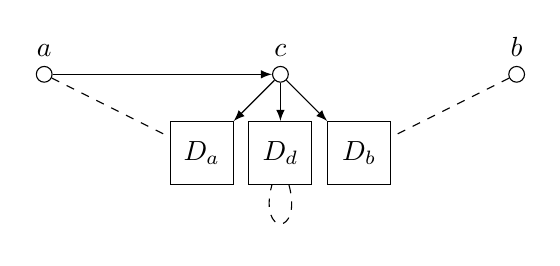
\begin{tikzpicture}
      [
      point/.style={circle,draw,inner sep=0pt,minimum size=2mm},
      collection/.style={rectangle,draw,inner sep=0pt,minimum height=8mm, minimum width= 8mm}
      ]
      \node (a) at (0,1) [point, label=above:$a$] {};
      \node (b) at (6,1) [point, label=above:$b$] {};
      \node (c) at (3,1) [point, label=above:$c$] {};
      \node (Da) at (2,0) [collection] {$D_a$};
      \node (Db) at (4,0) [collection] {$D_b$};
      \node (Dd) at (3,0) [collection] {$D_d$};
      \draw [-latex] (c) to (Da);
      \draw [-latex] (a) to (c);
      \draw [-latex] (c) to (Db);
      \draw [-latex] (c) to (Dd);
      \draw [dashed] (a) to (Da);
      \draw [dashed] (b) to (Db);
      \draw [dashed, loop below] (Dd) to (Dd);
    \end{tikzpicture}
    \caption{The inductive case of a $V_2$ construction.
    Boxes represents sets of vertices.
    An edge between a vertex and a box represents a set of edges from the vertex to each of the vertices in the set.}
    \label{fig:v2_situation}
  \end{figure}
  \FloatBarrier
  The inductive part of the $V_2$ definition (\ref{eq:V2_IS}) reveals two properties of the sets $D_b$, $D_a$ and $D_d$:
  \begin{itemize}
    \item The set $D_b$ is nonempty, since $\exists d \in N(c): V_2(d,b)$.
    \item $D_b \cup D_a \cup D_d = D$, since $\forall d \in N(c): V_2(d,b) \vee V_2(d,a) \vee V_2(d,d)$.
  \end{itemize}
  The induction hypothesis lets us assume the provability of the following sets of NAND-clauses:
  $\{ \ol{db} \;|\; d \in D_b \},\{ \ol{da} \;|\; d \in D_a \},\{ \ol{d} \;|\; d \in D_d \}$.
  Inserting these clauses into the incomplete proof from Figure~\ref{fig:proof_v2_partial} results the following proof:\par
  \begin{figure}[!h]
    \centering
    \begin{prooftree*}
      \Hypo{\ol{ac}}
      \Hypo{ \{ \ol{db} \;|\; d \in D_b \} }
      \Hypo{ \{ \ol{da} \;|\; d \in D_a \} }
      \Hypo{ \{ \ol{d} \;|\; d \in D_d \} }
      \Infer[right label=$cD$]4{\ol{ab}}
    \end{prooftree*}
    \caption{}
    \label{fig:proof_v2}
  \end{figure}
  The nonemptiness of $D_b$ gives us the existence of a $b$ in the premise, while he fact that $D_b \cup D_a \cup D_d = D$ guarantees that each atom in the OR-clause $D$ has a match in a NAND-clause.

  The proof is thus valid, finishing the inductive step and ultimately proving the fact that $V_2(a,b) \Rightarrow \;\vdash \ol{ab}$.
\end{proof}
Having that $V_2$ satisfies implication (1), if one could show that it also satisfies implication (2), the consequences would be considerable.
It would mean that any provable binary NAND-clause would have a proof that in each step combined a set of already proved binary NAND-clauses with an axiom.
Any provable NAND-clause could in other words be constructed by adding one fresh axiom at every step, hinting at a possible normal form of proofs in Neg.

Unfortunately, $V_2$ does \textit{not} satisfy implication (2).
The vertices $a$ and $b$ in the graph presented below will not be related by $V_2$, but $\ol{ab}$ is still provable in Neg.
The graph will thus act as a counterexample for implication (2).\par
\begin{figure}[!h]
  \centering
  \begin{tikzpicture}
    [
    point/.style={circle,draw,inner sep=0pt,minimum size=2mm}
    ]
    \node (a) at (0,4) [point, label=left:$a$] {};
    \node (x) at (1,3) [point, label=right:$x$] {};
    \node (y) at (1,2) [point, label=right:$y$] {};
    \node (z) at (1,1) [point, label=right:$z$] {};
    \node (c1) at (0,0) [point, label=left:$c_1$] {};
    \node (c2) at (2,0) [point, label=right:$c_2$] {};
    \node (b) at (2,4) [point, label=right:$b$] {};
    \draw [-latex] (a) to (c1);
    \draw [-latex] (a) to (x);
    \draw [-latex] (x) to (y);
    \draw [-latex] (y) to (z);
    \draw [-latex] (z) to (c1);
    \draw [-latex] (z) to (c2);
    \draw [-latex] (b) to (c2);

    \node (e1) [below left=6mm and 4mm of c1]  {};
    \node (e2) [below=8mm of c1] {};
    \node (e3) [below right=6mm and 4mm of c1] {};
    \draw [dashed] (e1) to (c1);
    \draw [dashed] (e2) to (c1);
    \draw [dashed] (e3) to (c1);

    \node (e1) [below left=6mm and 4mm of c2]  {};
    \node (e2) [below=8mm of c2] {};
    \node (e3) [below right=6mm and 4mm of c2] {};
    \draw [dashed] (e1) to (c2);
    \draw [dashed] (e2) to (c2);
    \draw [dashed] (e3) to (c2);
  \end{tikzpicture}
  \caption{}
  \label{fig:v2_counter_graph}
\end{figure}
\FloatBarrier
Given the above graph, $\ol{ab}$ can be proven like follows:\par
\begin{figure}[!h]
  \centering
  \begin{prooftree*}
    \Hypo{\ol{ax}}
    \Hypo{\ol{yz}}
    \Infer[left label=$xy$]2{\ol{az}}
    \Hypo{\ol{ac_1}}
    \Hypo{\ol{bc_2}}
    \Infer[right label=$zc_1c_2$]3{\ol{ab}}
  \end{prooftree*}
  \caption{}
  \label{fig:v2_counter_proof}
\end{figure}
To show that the graph in Figure~\ref{fig:v2_counter_graph} is not an instance of $V_2$ demands a closer look at the graph.

Assume $V_2(a,b)$.
Since $a$ and $b$ are not connected by an edge, their relation has to be an instance of the inductive step.
Because of the non-emptiness requirement, $\exists c \in N(a):\exists d \in N(c): V_2(d,b)$ from the $V_2$ definition, either $a$  must have a successor $c$ which again has a successor $d$ such that $V_2(d,b)$ or $b$ must have a successor $c$ which again has a successor $d$ such that $V_2(d,a)$.

The vertices $a$ and $b$ have a total of 3 successors, 2 of which only branch off to irrelevant vertices and therefore are unable to satisfy the non-emptiness requirement.
The last successor is the vertex $x$, which only has one successor, vertex $y$.\par
\begin{figure}[!h]
  \centering
  \begin{tikzpicture}
    [
    point/.style={circle,draw,inner sep=0pt,minimum size=2mm},
    one/.style={fill=black}
    ]
    \node (a) at (0,4) [point, label=left:$a$] {};
    \node (x) at (1,3) [point, label=right:$x$] {};
    \node (y) at (1,2) [point,one, label=right:$y$] {};
    \node (z) at (1,1) [point, label=right:$z$] {};
    \node (c1) at (0,0) [point,one, label=left:$c_1$] {};
    \node (c2) at (2,0) [point, label=right:$c_2$] {};
    \node (b) at (2,4) [point,one, label=right:$b$] {};
    \draw [-latex] (a) to (c1);
    \draw [-latex] (a) to (x);
    \draw [-latex] (x) to (y);
    \draw [-latex] (y) to (z);
    \draw [-latex] (z) to (c1);
    \draw [-latex] (z) to (c2);
    \draw [-latex] (b) to (c2);

    \node (e1) [below left=6mm and 4mm of c1]  {};
    \node (e2) [below=8mm of c1] {};
    \node (e3) [below right=6mm and 4mm of c1] {};
    \draw [dashed] (e1) to (c1);
    \draw [dashed] (e2) to (c1);
    \draw [dashed] (e3) to (c1);

    \node (e1) [below left=6mm and 4mm of c2]  {};
    \node (e2) [below=8mm of c2] {};
    \node (e3) [below right=6mm and 4mm of c2] {};
    \draw [dashed] (e1) to (c2);
    \draw [dashed] (e2) to (c2);
    \draw [dashed] (e3) to (c2);
  \end{tikzpicture}
  \caption{}
  \label{fig:v2_counter_assignment}
\end{figure}
\FloatBarrier
The above solution shows us by soundness of Neg that $\ol{yb}$ is unprovable, and therefore by implication (1) that $y$ and $b$ cannot be $V_2$-related.
Since none of the successors of $a$ and $b$ satisfies the non-emptiness requirement, they also are not $V_2$ related.
We can therefore conclude that $V_2$ does not satisfy implication (2).

\subsection{The $V_3$ construction}
\label{sub:The V3 construction}
Now, in what way can $V_2$ be generalized in order to include the graph in Figure~\ref{fig:v2_counter_graph}?
Looking at the proof in Figure~\ref{fig:proof_v2}, we see that the axiomatic NAND-clause $\ol{ac}$ is a crucial part of the premise, representing the $c \in N(a)$ in the definition of $V_2$.
Observe that a case where $\ol{ac}$ is non-axiomatic would not invalidate this rule application.
In other words, the vertex $c$ from the $V_2$ definition does not necessarily need to be in the neighborhood of $a$, they only need to be in a $V_2$-relation.

Based on this observation, we define the construction $V_3$ which is a generalization of $V_2$.
Like in the definitions of $V_1$ and $V_2$, $a$ and $b$ are vertices from $G$.
\begin{align}
  \textbf{(BC):}&\quad N(a,b) \vee N(b,a) &\Rightarrow V_3(a,b)\label{eq:V3_BC}\\
  \textbf{(IS):}&\quad \exists c \in G:
  \left ( \begin{tabular}{l}
  $\exists d \in N(c) \cup \{ c \} : V_3(d,a) \quad \wedge$\\
  $\exists d \in N(c) \cup \{ c \} : V_3(d,b) \quad \wedge$\\
  $\forall d \in N(c) \cup \{ c \} : V_3(d,a) \vee V_3(d,b) \vee V_3(d,d)$
  \end{tabular} \right )
  &\Rightarrow V_3(a,b)\label{eq:V3_IS}
\end{align}
$V_2$ required $a$ to have an edge to $c$.
We are now treating $c$ just like its successors by requiring it to be in $V_3$-relation to either $a$, $b$ or itself.
Requiring $a$ to be in $V_3$-relation to some vertex in $N(c) \cup \{ c \}$ is now what ensures the inclusion of $a$ in the proof.

Looking back at the graph from Figure~\ref{fig:v2_counter_graph}, we see that vertex $z$ is clearly $V_3$-related to $a$ while its successors, $c_1$ and $c_2$, are $V_3$-related to $a$ and $b$, respectively.
The vertices $a$ and $b$ are thus $V_3$-related.

Implication (1) for $V_3$ is proven in more or less the same way as we proved implication (1) for $V_2$ in Section~\ref{sub:The V2 construction}.
Therefore, only a condensed version will be shown here:
\begin{proof}
  Given a graph $G$ with two vertices $a$ and $b$ such that $V_3(a,b)$:

  Base case: Same as in $V_2$ proof.

  Inductive step: Let $D = N(c) \cup \{ c \}$ and let $D_a$, $D_b$ and $D_d$ denote the same sets as in the $V_2$ proof.
  The definition of $V_3$ tells us that both $D_a$ and $D_b$ are nonempty.
  This fact together with the fact that $D = D_a \cup D_b \cup D_d$ lets us form the following proof:\par
  \begin{figure}[!h]
    \centering
    \begin{prooftree*}
      \Hypo{ \{ \ol{da} \;|\; d \in D_a \} }
      \Hypo{ \{ \ol{db} \;|\; d \in D_b \} }
      \Hypo{ \{ \ol{d} \;|\; d \in D_d \} }
      \Infer[right label=$D$]3{\ol{ab}}
    \end{prooftree*}
    \caption{}
    \label{fig:proof_v3}
  \end{figure}
  No assumptions was made on the vertices $a$ and $b$, so we can conclude that $V_3(a,b)~\Rightarrow~\;\vdash~\ol{ab}$.
\end{proof}
\subsection{$V_3$ and implication (2)}
\label{sub:V3 and implication 2}
Just like with $V_2$, if $V_3$ also satisfies implication (2), it has some considerable consequences for our proof system, Neg.
Figure~\ref{fig:proof_v3} shows that if two vertices $a$ and $b$ are $V_3$-related, not only is $\ol{ab}$ provable in Neg, it is provable in such a way that the premise of the last rule application contains binary NAND-clauses only (the proof has a \textit{binary root}).

If $V_3$ satisfies implication (1) and (2), then for any provable binary NAND-clause $\ol{ab}$, by implication (1) and (2), it has a proof with a binary root.
Applying now the same reasoning on all of the binary NAND-clauses in its premise, we get that all of these also have proofs with binary roots.
Doing this repeatedly throughout the whole proof of $\ol{ab}$ ultimately gives us a proof containing exclusively binary NAND-clauses.
Implication (2) thus gives us that for any provable binary NAND-clause there exists a proof in Neg with binary NAND-clauses only.
We will however see that implication (2) does \textit{not} hold for $V_3$.\par

The graph in Figure~\ref{fig:v3_counter_graph} provides a provable NAND-clause $\ol{ab}$, but is not an instance of $V_3$.

The graph is admittedly a bit over-simplified.
Even though the vertices $y_1$, $y_2$ and $c_2$ are depicted like sinks, we will be treating them as initial vertices of (non-depicted) disjoint rays.
We will however not consider the clauses corresponding to the elements of these rays, since these are not going to contribute to our argument.
\begin{figure}[!h]
  \centering
  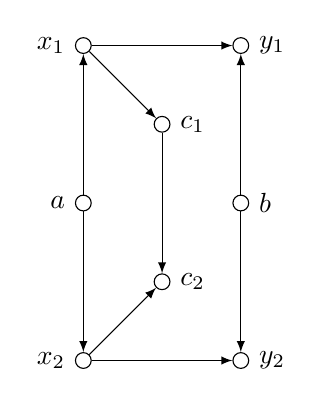
\begin{tikzpicture}
    [
    point/.style={circle,draw,inner sep=0pt,minimum size=2mm}
    ]
    \node (a) at (0,2) [point,label=left:$a$] {};
    \node (x1) at (0,4) [point,label=left:$x_1$] {};
    \node (x2) at (0,0) [point,label=left:$x_2$] {};
    \node (b) at (2,2) [point,label=right:$b$] {};
    \node (y1) at (2,4) [point,label=right:$y_1$] {};
    \node (y2) at (2,0) [point,label=right:$y_2$] {};
    \node (c1) at (1,3) [point,label=right:$c_1$] {};
    \node (c2) at (1,1) [point,label=right:$c_2$] {};
    \draw [-latex] (a) to (x1);
    \draw [-latex] (a) to (x2);
    \draw [-latex] (b) to (y1);
    \draw [-latex] (b) to (y2);
    \draw [-latex] (x1) to (y1);
    \draw [-latex] (x1) to (c1);
    \draw [-latex] (x2) to (y2);
    \draw [-latex] (x2) to (c2);
    \draw [-latex] (c1) to (c2);
  \end{tikzpicture}
  \caption{}
  \label{fig:v3_counter_graph}
\end{figure}
\FloatBarrier
Here is one way to prove $\ol{ab}$ in Neg given the graph theory from Figure~\ref{fig:v3_counter_graph}:\par
\begin{figure}[!h]
  \centering
  \begin{prooftree*}
    \Hypo{\ol{ax_2}}
    \Hypo{\ol{by_2}}
    \Hypo{\ol{c_1c_2}}
    \Infer[left label = $x_2y_2c_2$]3{\ol{abc_1}}
    \Hypo{\ol{ax_1}}
    \Hypo{\ol{by_1}}
    \Hypo{\ol{c_1c_2}}
    \Infer[right label = $x_1y_1c_1$]3{\ol{abc_2}}
    \Infer[left label = $c_1c_2$]2{\ol{ab}}
  \end{prooftree*}
  \caption{}
  \label{fig:v3_counter_proof}
\end{figure}
\FloatBarrier
Now, if implication (2) holds for $V_3$, we would expect $a$ and $b$ to be $V_3$-related in the above graph.
In other words, we would expect there to be a third vertex in the graph such that it and each of its successors are $V_3$-related to either $a$, $b$ or itself and such that at least one of them is $V_3$-related to $a$ and one to $b$.
This can be shown to be impossible.

Consider the following six solutions of the graph:\par
\begin{figure}[!h]
  \centering
  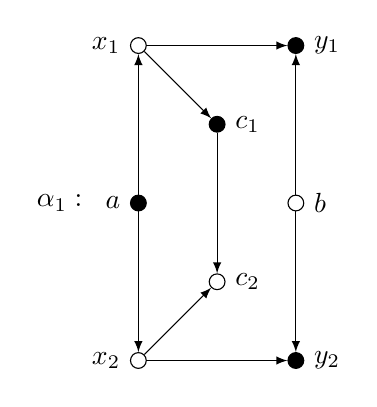
\begin{tikzpicture}
    [
    point/.style={circle,draw,inner sep=0pt,minimum size=2mm},
    one/.style={fill=black},
    collection/.style={thick,rectangle,draw,inner sep=0pt,minimum height=14mm, minimum width= 9mm}
    ]
    \node (label) at (-1,2) {$\alpha_1:$};
    \node (a) at (0,2) [point, one,label=left:$a$] {};
    \node (x1) at (0,4) [point,label=left:$x_1$] {};
    \node (x2) at (0,0) [point,label=left:$x_2$] {};
    \node (b) at (2,2) [point,label=right:$b$] {};
    \node (y1) at (2,4) [point, one,label=right:$y_1$] {};
    \node (y2) at (2,0) [point, one,label=right:$y_2$] {};
    \node (c1) at (1,3) [point, one,label=right:$c_1$] {};
    \node (c2) at (1,1) [point,label=right:$c_2$] {};
    \draw [-latex] (a) to (x1);
    \draw [-latex] (a) to (x2);
    \draw [-latex] (b) to (y1);
    \draw [-latex] (b) to (y2);
    \draw [-latex] (x1) to (y1);
    \draw [-latex] (x1) to (c1);
    \draw [-latex] (x2) to (y2);
    \draw [-latex] (x2) to (c2);
    \draw [-latex] (c1) to (c2);
  \end{tikzpicture}
  \hspace{5mm}
  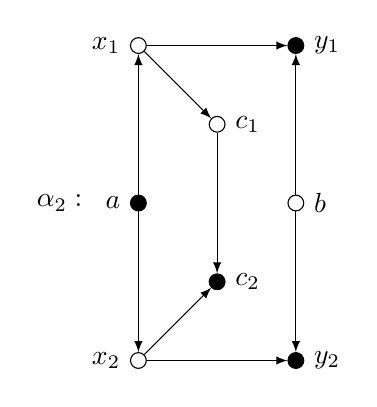
\begin{tikzpicture}
    [
    point/.style={circle,draw,inner sep=0pt,minimum size=2mm},
    one/.style={fill=black},
    collection/.style={thick,rectangle,draw,inner sep=0pt,minimum height=14mm, minimum width= 9mm}
    ]
    \node (label) at (-1,2) {$\alpha_2:$};
    \node (a) at (0,2) [point, one,label=left:$a$] {};
    \node (x1) at (0,4) [point,label=left:$x_1$] {};
    \node (x2) at (0,0) [point,label=left:$x_2$] {};
    \node (b) at (2,2) [point,label=right:$b$] {};
    \node (y1) at (2,4) [point, one,label=right:$y_1$] {};
    \node (y2) at (2,0) [point, one, label=right:$y_2$] {};
    \node (c1) at (1,3) [point,label=right:$c_1$] {};
    \node (c2) at (1,1) [point, one, label=right:$c_2$] {};
    \draw [-latex] (a) to (x1);
    \draw [-latex] (a) to (x2);
    \draw [-latex] (b) to (y1);
    \draw [-latex] (b) to (y2);
    \draw [-latex] (x1) to (y1);
    \draw [-latex] (x1) to (c1);
    \draw [-latex] (x2) to (y2);
    \draw [-latex] (x2) to (c2);
    \draw [-latex] (c1) to (c2);
  \end{tikzpicture}
  \hspace{5mm}
  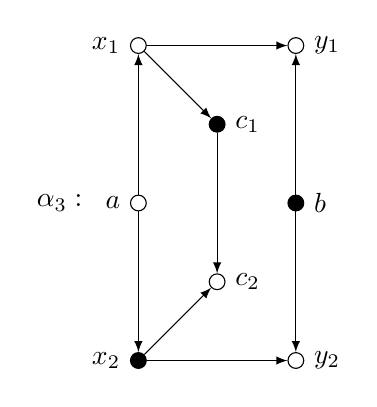
\begin{tikzpicture}
    [
    point/.style={circle,draw,inner sep=0pt,minimum size=2mm},
    one/.style={fill=black},
    collection/.style={thick,rectangle,draw,inner sep=0pt,minimum height=14mm, minimum width= 9mm}
    ]
    \node (label) at (-1,2) {$\alpha_3:$};
    \node (a) at (0,2) [point,label=left:$a$] {};
    \node (x1) at (0,4) [point,label=left:$x_1$] {};
    \node (x2) at (0,0) [point, one,label=left:$x_2$] {};
    \node (b) at (2,2) [point, one,label=right:$b$] {};
    \node (y1) at (2,4) [point,label=right:$y_1$] {};
    \node (y2) at (2,0) [point,label=right:$y_2$] {};
    \node (c1) at (1,3) [point, one,label=right:$c_1$] {};
    \node (c2) at (1,1) [point,label=right:$c_2$] {};
    \draw [-latex] (a) to (x1);
    \draw [-latex] (a) to (x2);
    \draw [-latex] (b) to (y1);
    \draw [-latex] (b) to (y2);
    \draw [-latex] (x1) to (y1);
    \draw [-latex] (x1) to (c1);
    \draw [-latex] (x2) to (y2);
    \draw [-latex] (x2) to (c2);
    \draw [-latex] (c1) to (c2);
  \end{tikzpicture}\\
  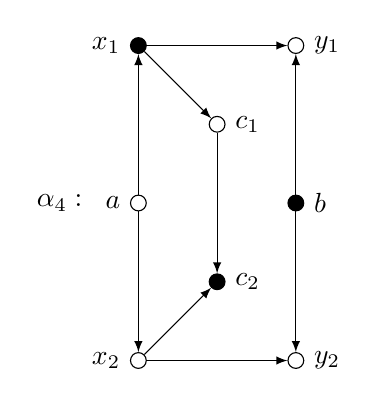
\begin{tikzpicture}
    [
    point/.style={circle,draw,inner sep=0pt,minimum size=2mm},
    one/.style={fill=black},
    collection/.style={thick,rectangle,draw,inner sep=0pt,minimum height=14mm, minimum width= 9mm}
    ]
    \node (label) at (-1,2) {$\alpha_4:$};
    \node (a) at (0,2) [point,label=left:$a$] {};
    \node (x1) at (0,4) [point, one,label=left:$x_1$] {};
    \node (x2) at (0,0) [point,label=left:$x_2$] {};
    \node (b) at (2,2) [point, one,label=right:$b$] {};
    \node (y1) at (2,4) [point,label=right:$y_1$] {};
    \node (y2) at (2,0) [point,label=right:$y_2$] {};
    \node (c1) at (1,3) [point,label=right:$c_1$] {};
    \node (c2) at (1,1) [point, one,label=right:$c_2$] {};
    \draw [-latex] (a) to (x1);
    \draw [-latex] (a) to (x2);
    \draw [-latex] (b) to (y1);
    \draw [-latex] (b) to (y2);
    \draw [-latex] (x1) to (y1);
    \draw [-latex] (x1) to (c1);
    \draw [-latex] (x2) to (y2);
    \draw [-latex] (x2) to (c2);
    \draw [-latex] (c1) to (c2);
  \end{tikzpicture}
  \hspace{5mm}
  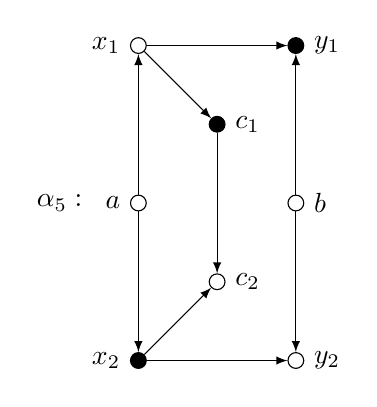
\begin{tikzpicture}
    [
    point/.style={circle,draw,inner sep=0pt,minimum size=2mm},
    one/.style={fill=black},
    collection/.style={thick,rectangle,draw,inner sep=0pt,minimum height=14mm, minimum width= 9mm}
    ]
    \node (label) at (-1,2) {$\alpha_5:$};
    \node (a) at (0,2) [point,label=left:$a$] {};
    \node (x1) at (0,4) [point,label=left:$x_1$] {};
    \node (x2) at (0,0) [point, one,label=left:$x_2$] {};
    \node (b) at (2,2) [point,label=right:$b$] {};
    \node (y1) at (2,4) [point, one, label=right:$y_1$] {};
    \node (y2) at (2,0) [point,label=right:$y_2$] {};
    \node (c1) at (1,3) [point, one,label=right:$c_1$] {};
    \node (c2) at (1,1) [point,label=right:$c_2$] {};
    \draw [-latex] (a) to (x1);
    \draw [-latex] (a) to (x2);
    \draw [-latex] (b) to (y1);
    \draw [-latex] (b) to (y2);
    \draw [-latex] (x1) to (y1);
    \draw [-latex] (x1) to (c1);
    \draw [-latex] (x2) to (y2);
    \draw [-latex] (x2) to (c2);
    \draw [-latex] (c1) to (c2);
  \end{tikzpicture}
  \hspace{5mm}
  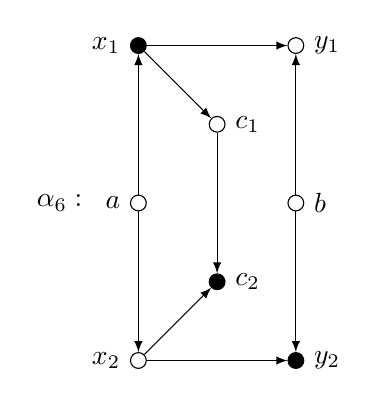
\begin{tikzpicture}
    [
    point/.style={circle,draw,inner sep=0pt,minimum size=2mm},
    one/.style={fill=black},
    collection/.style={thick,rectangle,draw,inner sep=0pt,minimum height=14mm, minimum width= 9mm}
    ]
    \node (label) at (-1,2) {$\alpha_6:$};
    \node (a) at (0,2) [point,label=left:$a$] {};
    \node (x1) at (0,4) [point, one, label=left:$x_1$] {};
    \node (x2) at (0,0) [point,label=left:$x_2$] {};
    \node (b) at (2,2) [point, label=right:$b$] {};
    \node (y1) at (2,4) [point,label=right:$y_1$] {};
    \node (y2) at (2,0) [point, one, label=right:$y_2$] {};
    \node (c1) at (1,3) [point,label=right:$c_1$] {};
    \node (c2) at (1,1) [point, one, label=right:$c_2$] {};
    \draw [-latex] (a) to (x1);
    \draw [-latex] (a) to (x2);
    \draw [-latex] (b) to (y1);
    \draw [-latex] (b) to (y2);
    \draw [-latex] (x1) to (y1);
    \draw [-latex] (x1) to (c1);
    \draw [-latex] (x2) to (y2);
    \draw [-latex] (x2) to (c2);
    \draw [-latex] (c1) to (c2);
  \end{tikzpicture}
  \caption{}
  \label{fig:v3_counter_solutions}
\end{figure}
\FloatBarrier
Given any pair of vertices $x,y$, if there exists a solution such that $x$ and $y$ are both assigned 1, then $\ol{xy}$ is not provable in Neg.
We get this from soundness.

The table in Figure~\ref{fig:v3_counter_table} shows what pairs of vertices can be 1 under the same solution and thus constitute a binary NAND-clauses unprovable in Neg.
A cell is filled with a reference to the solution, if any, exemplifying the case.
This relation is obviously symmetric, so we leave out the lower half of the table to ease readability.
\begin{figure}[!h]
  \centering
  \[\begin{array}{|c||c|c|c|c|c|c|c|c|}
    \hline
    & a & b & x_1 & x_2 & y_1 & y_2 & c_1 & c_2 \\ \hline\hline
    a & \alpha_1 & & & & \alpha_1 & \alpha_1 & \alpha_1 & \alpha_2 \\ \hline
    b &-& \alpha_4 & \alpha_4 & \alpha_3 & & & \alpha_3 & \alpha_4 \\ \hline
    x_1 &-&-& \alpha_4 & & & \alpha_6 & & \alpha_6 \\ \hline
    x_2 &-&-&-& \alpha_5 & \alpha_5 & & \alpha_5 & \\ \hline
    y_1 &-&-&-&-& \alpha_1 & \alpha_1 & \alpha_1 & \alpha_2 \\ \hline
    y_2 &-&-&-&-&-& \alpha_1 & \alpha_1 & \alpha_2 \\ \hline
    c_1 &-&-&-&-&-&-& \alpha_1 & \\ \hline
    c_2 &-&-&-&-&-&-&-& \alpha_4 \\ \hline
  \end{array}\]
  \caption{}
  \label{fig:v3_counter_table}
\end{figure}
\FloatBarrier
Two important observations are to be made from the above table:

First, for each vertex in the graph, there exists a solution where that vertex is assigned 1.
By soundness, no unary NAND-clause can therefore be proven in Neg under this theory.

Secondly, among the pairs above that are not shown to be unprovable, only two are not axioms: $\ol{ab}$ and $\ol{x_1x_2}$.
We are thus left with the following collection of 11 ``not-unprovable'' binary NAND-clauses:
\begin{align}
  \{\; \ol{ab},\; \ol{ax_1},\; \ol{ax_2},\; \ol{by_1},\; \ol{by_2},\; \ol{x_1x_2},\; \ol{x_1y_1},\; \ol{x_1c_1},\; \ol{x_2y_2},\; \ol{x_2c_2} \; \ol{c_1c_2}\; \}
\end{align}
By the definition of $V_3$ from (\ref{eq:V2_BC}) and (\ref{eq:V2_IS}), in order for $a$ and $b$ to be $V_3$-related, a vertex $c$ has to exist such that it and all its successors are $V_3$-related to either $a$, $b$ or itself and such that at least one of them is $V_3$-related to $a$ and one to $b$.

It turns out that none of the vertices in the graph satisfies this requirement.
$a$ and $b$ are therefore not $V_3$-related, and so implication (2) fails.
